%
% antennenAllgemein.tex 
%
% 
%
% !TEX root = ../../buch.tex
% !TEX encoding = UTF-8
%

\section{Antennen\label{antennen:antennenAllgemein}}


Antennen sind in der heutigen technologischen Welt unverzichtbar. Sie sind in zahlreichen Formen und Varianten in fast allen elektronischen Geräten zu finden. Ihre primäre Funktion besteht darin, elektromagnetische Wellen von einer leitungsgebundenen Form in freie Wellen im Raum zu verwandeln. Dieser Vorgang ist essenziell für die Kommunikation, da er die Übertragung von Signalen über große Distanzen ermöglicht. Ein weiterer entscheidender Aspekt von Antennen ist ihre Reziprozität: Sie können sowohl Signale senden als auch empfangen. Dabei wandeln sie freie Wellen aus dem Raum zurück in leitungsgebundene Wellen. Diese Fähigkeit macht Antennen zu einem grundlegenden Element der modernen Kommunikationstechnologie. Ohne sie wäre die drahtlose Übertragung von Daten und Signalen, wie wir sie heute kennen, undenkbar.

Eine genauere Erklärung von elektromagnetischen Wechselwirkungen findet der Leser im Kapitel \ref{chapter:maxwell},
welches sich mit den Maxwell-Gleichungen befasst. 
\subsection{Loop-Antennen\label{antennen:antennenAllgemein_loop}}


Eine Loop-Antenne hat eine recht simple Funktionsweise. Sie besteht aus einem Stück Draht wie in Abbildung \ref{antennen:loopAntenne} dargestellt. Die Loop-Antenne kann, nicht wie der Name impliziert, verschiedenste Formen annehmen. Durch den Leiter wird ein Signal geführt, das in der aufgespannten Fläche ein magnetisches Feld induziert. Dieses Feld wird durch Anpassung der Signalamplitude verändert. Eine solche Änderung kann als Information angesehen werden, die sich nun im freien Raum fortbewegt.

\begin{figure}
	\centering
	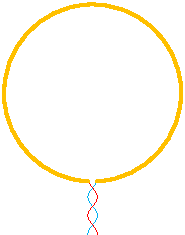
\includegraphics{papers/antennen/images/loopAntenne.pdf}
	\caption{Form einer typischen Loop-Antenne}
	\label{antennen:loopAntenne}
\end{figure}

\subsection{Eigenschaften\label{antennen:antennenEigenschaften}}
Der Wirkungsgrad
\begin{equation}
	\eta=\frac{P\textsubscript{rad}}{P\textsubscript{tot}},
	\label{antennen:Wirkungsgrad}
\end{equation}
auch Effizienz genannt, kann mittels der eingespeisten Gesamtleistung der Antenne $P\textsubscript{tot}$ und der abgestrahlten Leistung $P\textsubscript{rad}$ berechnet werden. Eine Leistung $P$ entspricht dem elektrischen Widerstand multipliziert mit der Stromstärke im Quadrat. Nach Vereinfachung ergibt sich, dass die Effizienz

\begin{equation}
	\eta=\frac{P\textsubscript{rad}}{P\textsubscript{tot}}=\frac{R\textsubscript{rad}\cdot{I^2}}{R\textsubscript{tot}\cdot{I^2}}=\frac{R\textsubscript{rad}\cdot{I^2}}{(R\textsubscript{rad}+R\textsubscript{loss})\cdot{I^2}}=\frac{R\textsubscript{rad}}{R\textsubscript{rad}+R\textsubscript{loss}}
	\label{antennen:Wirkungsgradkomplett}
\end{equation}
nur noch vom Verlustwiderstand und dem Strahlungswiderstand abhängig ist. $R\textsubscript{rad}$ und $R\textsubscript{loss}$ werden wie folgt definiert:
\begin{align}
	R_{\text{rad}} &= 31171 \Omega \cdot \bigg( \frac{A}{\lambda^2} \bigg)^2 \tag{20.3} \label{antennen:Rrad} \\
	R_{\text{loss}} &= \frac{\rho \cdot l}{r^2 \cdot \pi}. \tag{20.4} \label{antennen:Rloss}
\end{align}

Die Formel \eqref{antennen:Rrad} für die Berechnung des Strahlungswiderstands wurde aus Fachliteratur \cite{antennen:antennaTheory} übernommen, welche erklärt, dass die ``magische'' Konstante in \eqref{antennen:Rrad} durch elektrodynamische Gesetzte entsteht. Sie gilt für die verschiedensten Formen von Loop-Antennen, welche einen kleinen Umfang  $l$ < $\lambda$/10 aufweisen. $A$ wird hierbei als aufgespannte Fläche definiert, während $\lambda$ der Wellenlänge entspricht. Eine Wellenlänge 
\setcounter{equation}{4}

\begin{equation}
	\lambda = \frac{c}{f}
	\label{antennen:lambda}
\end{equation}
entspricht dem Verhältnis der materialspezifischen Lichtgeschwindigkeit $c$ und der Einsatzfrequenz $f$.
Der Verlustwiderstand wird aus dem spezifischen Widerstand $\rho$, dem Umfang $l$ und dem Leiterradius $r$ berechnet. Die Formeln \eqref{antennen:Rrad} und \eqref{antennen:Rloss} können in dieser Arbeit vereinfacht werden, da die Einsatzfrequenz und die Drahteigenschaften als konstant und gegeben angesehen werden können. Es resultieren die Ausdrücke 
\begin{align}
	R_{\text{rad}} &= k_{\text{1}} \cdot A^2 \tag{20.6} \label{antennen:Rrad_konst} \\
	R_{\text{loss}} &= k_{\text{2}} \cdot l \tag{20.7} \label{antennen:Rloss_konst}
\end{align}
für die beiden Widerstände. $k\textsubscript{1}$ und $k\textsubscript{2}$ werden als Konstanten betrachtet. Eingesetzt in \eqref{antennen:Wirkungsgradkomplett} ergibt sich
\setcounter{equation}{7}
\begin{equation}
	\eta=\frac{k\textsubscript{1}\cdot{A^2}}{k\textsubscript{1}\cdot{A^2}+{k\textsubscript{2}\cdot{l}}}=\frac{1}{1+\frac{k\textsubscript{2}\cdot{l}}{k\textsubscript{1}\cdot{A^2}}}
	\label{antennen:Wirkungsgradeingesetzt}
\end{equation}
für den Wirkungsgrad.
